
% !TeX root = master.tex

\hypertarget{tuning-reference}{%
\section{Tuning reference}\label{tuning-reference}}

This file documents the gain scheduling rules in \texttt{tuning.js}. The goal of this
section is not to justify every parameter choice, but to make it easy to connect the code
to the physical intent. For that reason, variable names refer directly to
\texttt{KALMAN\_TUNING} so the plots stay tied to the actual configuration. Plots are
generated by \texttt{scripts/plot\_tuning.py}.

\hypertarget{process-noise-vs-boat-length-acceleration-variance}{%
\subsection{Process noise vs boat length (acceleration
variance)}\label{process-noise-vs-boat-length-acceleration-variance}}

We scale the base acceleration variance by boat length so longer boats
respond more slowly. For lengths shorter than the anchor, we do not
increase the base value.

\begin{flalign}
\hspace{5em}q &= \text{baseQ} \left(\frac{L_0}{\max(L_0, L)}\right)^2 && \left[\mathrm{m^2/s^4}\right] \label{eq:tuning:q-length}
\end{flalign}
In \eqref{eq:tuning:q-length}, \(q\) is the adjusted acceleration variance and
\(\text{baseQ}\) is \texttt{KALMAN\_TUNING.processNoise.baseAccelerationVariance}. The
anchor length \(L_0\) is
\texttt{KALMAN\_TUNING.processNoise.baseBoatLengthMeters}, and \(L\) is the current boat
length.

\begin{figure}
\centering
\includegraphics{./plots/gain-q-length.pdf}
\caption{Process noise vs boat length}
\end{figure}

\hypertarget{speed-scale-from-recent-max-speed}{%
\subsection{Speed scale from recent max
speed}\label{speed-scale-from-recent-max-speed}}

The process noise is further scaled by recent max speed (not
instantaneous speed). We use the maximum speed over a recent window to
capture the boat's potential to accelerate even if it is currently slow.

\begin{flalign}
\hspace{5em}\text{speedScale} &= \frac{\max(v^*_{\text{kn}}, v_{\min})}{v_{\text{anchor}}} && \left[1\right] \label{eq:tuning:speed-scale}
\end{flalign}
In \eqref{eq:tuning:speed-scale}, \(\text{speedScale}\) is dimensionless,
\(v^*_{\text{kn}}\) is the recent maximum speed in knots over the window
\texttt{KALMAN\_TUNING.processNoise.speedScale.recentMaxSpeedWindowSeconds}, \(v_{\min}\)
is \texttt{KALMAN\_TUNING.processNoise.speedScale.minKnots}, and
\(v_{\text{anchor}}\) is
\texttt{KALMAN\_TUNING.processNoise.speedScale.anchorKnots}.

\begin{figure}
\centering
\includegraphics{./plots/gain-speed-scale.pdf}
\caption{Speed-based gain scale}
\end{figure}

\hypertarget{imu-gravity-low-pass-vs-boat-length}{%
\subsection{IMU gravity low-pass vs boat
length}\label{imu-gravity-low-pass-vs-boat-length}}

The gravity estimate is low-pass filtered so the down axis stays stable
in waves. We scale the low-pass factor by boat length: larger boats get
a slower response.

\begin{flalign}
\hspace{5em}\alpha &= \text{clamp}\left(\alpha_0 \sqrt{\frac{L_0}{\max(L_0, L)}},\; \alpha_{\min},\; \alpha_{\max}\right) && \left[1\right] \label{eq:tuning:gravity-alpha}
\end{flalign}
In \eqref{eq:tuning:gravity-alpha}, \(\alpha\) is the gravity low-pass factor,
\(\alpha_0\) is \texttt{KALMAN\_TUNING.imu.gravityLowPass.baseAlpha}, \(L_0\) is
\texttt{KALMAN\_TUNING.imu.gravityLowPass.baseBoatLengthMeters}, \(\alpha_{\min}\) is
\texttt{KALMAN\_TUNING.imu.gravityLowPass.minAlpha}, and \(\alpha_{\max}\) is
\texttt{KALMAN\_TUNING.imu.gravityLowPass.maxAlpha}.

\begin{figure}
\centering
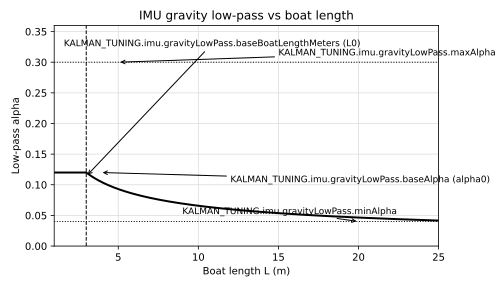
\includegraphics{./plots/gain-gravity-alpha.pdf}
\caption{IMU gravity low-pass vs boat length}
\end{figure}

\hypertarget{process-noise-anisotropy-forward-vs-lateral}{%
\subsection{Process noise anisotropy (forward vs
lateral)}\label{process-noise-anisotropy-forward-vs-lateral}}

Boats change speed much more easily along their heading than sideways.
We encode that by scaling the lateral acceleration variance as a fixed
fraction of the forward variance:

\begin{flalign}
\hspace{5em}q_{\text{lateral}} &= \rho\,q_{\text{forward}} && \left[\mathrm{m^2/s^4}\right] \label{eq:tuning:q-lateral}
\end{flalign}
In \eqref{eq:tuning:q-lateral}, \(q_{\text{lateral}}\) is the lateral acceleration
variance, \(q_{\text{forward}}\) is the forward acceleration variance, and \(\rho\) is
\texttt{KALMAN\_TUNING.imu.lateralVarianceRatio}.
